\documentclass[12pt,a4paper]{article}

% Packages essentiels
\usepackage[utf8]{inputenc}
\usepackage[T1]{fontenc}
\usepackage[french]{babel}
\usepackage{geometry}
\usepackage{graphicx}
\usepackage{hyperref}
\usepackage{amsmath}
\usepackage{amsfonts}
\usepackage{amssymb}
\usepackage{enumitem}
\usepackage{float}
\usepackage{caption}
\usepackage{subcaption}
\usepackage{listings}
\usepackage{xcolor}
\usepackage{fancyhdr}
\usepackage{titlesec}
\usepackage{datetime2}

% Configuration de la page
\geometry{
    left=2.5cm,
    right=2.5cm,
    top=3cm,
    bottom=3cm
}

% Configuration des hyperliens
\hypersetup{
    colorlinks=false,
    hidelinks=true,
    pdftitle={Contrôle gestuel d'une application vidéo par vision artificielle},
    pdfauthor={GOAREGUER Maël, AKKAYA Garip, BAUDART Alexandre, POTIN Léa}
}

% Configuration des en-têtes et pieds de page
\pagestyle{fancy}
\fancyhf{}
\fancyhead[L]{\leftmark}
\fancyhead[R]{\thepage}
\fancyfoot[C]{Rapport final - Vision numérique (GIF-7001)}

% Configuration des titres
\titleformat{\section}
{\Large\bfseries}
{\thesection}{1em}{}
[\titlerule]

\titleformat{\subsection}
{\large\bfseries}
{\thesubsection}{1em}{}

% Configuration pour la table des matières
\usepackage{tocloft}
\renewcommand{\cftsecleader}{\cftdotfill{\cftdotsep}}

% Configuration des listes
\setlist[itemize]{leftmargin=*,itemsep=0.5em}
\setlist[enumerate]{leftmargin=*,itemsep=0.5em}

% Configuration du code (si nécessaire)
\lstset{
    basicstyle=\ttfamily\small,
    breaklines=true,
    frame=single,
    language=Python,
    numbers=left,
    numberstyle=\tiny\color{gray}
}

% Informations du document
\title{%
    \vspace{-2cm}
    \textbf{Contrôle gestuel d'une application vidéo\\par vision artificielle}
    \vspace{0.5cm}
}
\author{%
    GOAREGUER Maël - 537407419\\
    AKKAYA Garip - 537399808\\
    BAUDART Alexandre - 537344920\\
    POTIN Léa - 537396798
}
\date{%
    \vspace{0.5cm}
    Date de remise : 11 décembre 2025\\
    \vspace{0.3cm}
    Cours : Vision numérique (GIF-7001)\\
    Professeur : Robert Bergevin
}

\begin{document}

\maketitle
\thispagestyle{empty}
\newpage

\tableofcontents
\newpage

\section{Mise en contexte et description de la solution réalisée}

L'interaction homme-machine évolue rapidement vers des interfaces plus naturelles et intuitives, dans le but de réduire la complexité d'utilisation et d'améliorer l'expérience utilisateur. Parmi ces interfaces, le contrôle gestuel s'impose comme une alternative prometteuse aux dispositifs classiques tels que la souris, le clavier ou la télécommande. Initialement popularisé par le domaine du jeu vidéo et les systèmes immersifs, le contrôle gestuel trouve aujourd'hui des applications dans la vidéo, la domotique, la santé, et l'industrie. En particulier, les lecteurs vidéo bénéficient directement de cette technologie, permettant à l'utilisateur de naviguer dans le contenu multimédia sans contact physique, de manière fluide et intuitive, et d'interagir tout en effectuant d'autres tâches. Ce type de contrôle offre non seulement une expérience plus immersive mais améliore également l'accessibilité pour les utilisateurs présentant des limitations motrices.

Le projet réalisé vise à développer un système de reconnaissance gestuelle capable de contrôler un lecteur vidéo via une webcam. L'objectif principal est de permettre à l'utilisateur d'interagir avec la vidéo par de simples mouvements de la main, sans nécessiter de contact physique avec le périphérique. Notre solution repose sur une architecture logicielle modulaire développée en Python, intégrant des technologies de vision par ordinateur et des outils spécialisés de détection de mouvements. L'architecture se compose de plusieurs modules principaux :

\subsection{Architecture technique}

\begin{itemize}
    \item \textbf{Interface utilisateur} : Application PySide6 offrant une interface graphique claire et intuitive, intégrant un lecteur vidéo et des menus de configuration.
    
    \item \textbf{Capture vidéo} : Module OpenCV pour la capture et le prétraitement des images en temps réel (conversion en RGB, redimensionnement, réglage de la résolution et du taux de rafraîchissement).
    
    \item \textbf{Détection de mains} : Moteur MediaPipe Hands pour la détection et le suivi des mains, avec extraction de 21 landmarks par main et distinction entre les mains gauche et droite.
    
    \item \textbf{Traitement des gestes} : Système de reconnaissance de gestes basé sur des règles heuristiques, calculant distances et angles entre les articulations pour identifier les postures.
    
    \item \textbf{Contrôle de l'application} : Interface de communication avec le lecteur vidéo intégré, permettant la lecture/pause, l'avance ou le retour rapide, le réglage du volume et le mode plein écran.
\end{itemize}

\subsection{Fonctionnalités réalisées}

\begin{itemize}
    \item Détection et suivi en temps réel des mains dans le flux vidéo.
    \item Reconnaissance de six gestes prédéfinis : ``play/pause'', ``avancer'', ``reculer'', ``volume up'', ``volume down'' et ``fullscreen''.
    \item Interface utilisateur avec configuration des paramètres de détection et visualisation des landmarks en temps réel.
    \item Système de logging complet pour le débogage et l'optimisation.
    \item Architecture modulaire facilitant l'ajout de nouveaux gestes et fonctionnalités.
    \item Système de métriques permettant l'évaluation des performances et la création de matrices de confusion.
\end{itemize}

L'utilisation de MediaPipe présente plusieurs avantages : rapidité d'exécution garantissant un traitement en temps réel, précision élevée dans la détection grâce aux 21 points de repère par main, et intégration simplifiée via des modèles pré-entraînés. L'architecture modulaire assure une maintenance facile et permet l'évolution du système sans impacter les modules existants.

\begin{figure}[H]
    \centering
    \begin{subfigure}{0.48\textwidth}
        \centering
        \includegraphics[width=\textwidth]{../images/gestes_lecture_navigation.png}
        \caption{Gestes de lecture (play/pause) et navigation (avancer/reculer)}
        \label{fig:gestes_lecture}
    \end{subfigure}
    \hfill
    \begin{subfigure}{0.48\textwidth}
        \centering
        \includegraphics[width=\textwidth]{../images/gestes_volume_fullscreen.png}
        \caption{Gestes de volume (volume up/volume down) et plein écran (fullscreen)}
        \label{fig:gestes_volume}
    \end{subfigure}
    \caption{Illustration des gestes reconnus par le système}
    \label{fig:gestes}
\end{figure}

\subsection{Approfondissement technique}

Le module de capture vidéo utilise OpenCV pour acquérir les images à 30 FPS en résolution 1280×720. Chaque image est prétraitée avant d'être transmise au moteur MediaPipe. Le moteur identifie les positions des mains et calcule les distances et angles entre les articulations pour déterminer la posture. Ces mesures servent ensuite au système de reconnaissance heuristique pour classifier les gestes. Un mécanisme de ``debounce'' empêche les déclenchements multiples lors de mouvements rapides ou tremblants. L'interface PySide6 visualise les landmarks et offre un retour en temps réel, permettant à l'utilisateur de confirmer visuellement que le geste a bien été reconnu.

\subsection{Scénario d'utilisation typique}

L'utilisateur lance l'application, active la capture vidéo, et interagit avec le lecteur. Pour mettre la vidéo en pause, il effectue un geste simple de la main. Le geste est détecté et confirmé par un retour visuel sur l'interface, et la vidéo se met instantanément en pause. De même, l'utilisateur peut avancer rapidement, reculer, ajuster le volume ou passer en plein écran uniquement avec des gestes naturels, sans toucher le clavier ou la souris.

\subsection{Comparaison avec d'autres solutions}

Contrairement aux systèmes utilisant des capteurs externes (Kinect, Leap Motion) ou des modèles d'apprentissage automatique complexes, notre solution purement logicielle repose sur une webcam standard et MediaPipe. Cela la rend facilement déployable sur n'importe quel poste, avec une latence faible et une précision suffisante pour les commandes vidéo courantes, tout en restant extensible pour des fonctionnalités futures.

\section{Justification des choix de design finaux}

\subsection{Choix technologiques}

\subsubsection{Python comme langage principal}

Python a été choisi pour sa richesse en bibliothèques de vision par ordinateur et d'apprentissage automatique (TensorFlow, PyTorch, MediaPipe).

\subsubsection{PySide6 pour l'interface utilisateur}

PySide6 offre une interface multiplateforme, une intégration avec le système d'exploitation, et une excellente performance pour les applications de traitement vidéo en temps réel. PySide6 est utilisé pour créer l'interface graphique principale, gérer l'affichage vidéo, et implémenter les dialogues de métriques. Les signaux de Qt permettent une communication asynchrone entre les threads de capture vidéo et l'interface utilisateur, garantissant une réactivité optimale même lors du traitement intensif des frames vidéo en même temps que la webcam.

\subsubsection{MediaPipe pour la détection de mains et la reconnaissance de gestes}

MediaPipe Hands a été choisi pour sa capacité à détecter et suivre les mains en temps réel avec une latence faible. La bibliothèque fournit 21 points de repère (landmarks) par main, permettant une analyse précise de la posture des doigts. Ces landmarks sont utilisés pour calculer les distances et angles entre les articulations, formant la base d'un système de classification de gestes basé sur des règles heuristiques.

\subsubsection{OpenCV pour la capture vidéo et le traitement d'images}

OpenCV est utilisé pour la capture vidéo depuis la webcam via l'interface VideoCapture, permettant la configuration de la résolution et du taux de rafraîchissement. OpenCV fournit une interface robuste et optimisée pour la capture vidéo, avec support natif pour différentes sources (webcam, fichiers vidéo) et formats de résolution.

\subsubsection{NumPy pour les calculs géométriques}

NumPy est utilisé pour effectuer les calculs de distances euclidiennes entre les landmarks de MediaPipe, permettant de déterminer l'état des doigts (tendus/repliés) et de calculer les ratios de mouvement horizontal/vertical nécessaires à la classification des gestes.

\subsection{Architecture modulaire}

L'architecture modulaire adoptée sépare clairement les responsabilités :

\begin{itemize}
    \item \textbf{Module video} : Gestion de la capture vidéo
    \item \textbf{Module engines} : Moteurs de traitement (MediaPipe)
    \item \textbf{Module processing} : Processeurs de flux vidéo
    \item \textbf{Module ui} : Interface utilisateur
    \item \textbf{Module utils} : Utilitaires (configuration, logging, métriques)
\end{itemize}

Cette séparation facilite les tests unitaires, la maintenance, et l'ajout de nouvelles fonctionnalités.

\subsection{Configuration flexible}

L'utilisation de fichiers YAML pour la configuration permet une personnalisation facile des paramètres sans modification du code source, facilitant l'adaptation à différents environnements et cas d'usage. Les paramètres configurables incluent les seuils de confiance de détection, les résolutions vidéo, et les paramètres de reconnaissance de gestes.

\section{Résultats finaux obtenus}

\subsection{Détection de mains}

Le système de détection a été implémenté et permet d'identifier les mains en temps réel dans le flux vidéo. Il affiche les 21 landmarks par main avec leurs connexions, traite les images à 30 FPS en résolution 1280×720 et gère différents seuils de détection et paramètres configurables. Le système supporte la détection de plusieurs mains simultanément et distingue correctement les mains gauche et droite.

\subsection{Interface utilisateur}

Une interface graphique a été développée pour visualiser le flux vidéo annoté en direct. Elle intègre des contrôles permettant d'activer ou désactiver la détection MediaPipe, un menu de paramètres pour ajuster la configuration, un visualiseur de journaux d'exécution et un système d'aide contextuelle. L'interface permet également de charger et contrôler des fichiers vidéo avec un lecteur intégré.

\subsection{Reconnaissance de gestes}

Un système de reconnaissance de gestes basé sur des règles heuristiques a été implémenté. Le système analyse les positions relatives des landmarks de MediaPipe pour reconnaître six gestes prédéfinis :

\begin{itemize}
    \item \textbf{TOGGLE\_PLAY\_PAUSE} : Main plate avec tous les doigts tendus et collés
    \item \textbf{FULLSCREEN} : Main plate avec tous les doigts tendus et écartés
    \item \textbf{AVANCER} : Index pointé vers la gauche (mouvement horizontal)
    \item \textbf{RECULER} : Index pointé vers la droite (mouvement horizontal)
    \item \textbf{VOLUME\_UP} : Index pointé vers le haut (mouvement vertical)
    \item \textbf{VOLUME\_DOWN} : Index pointé vers le bas (mouvement vertical)
\end{itemize}

Le système utilise des seuils et ratios calculés à partir des distances entre landmarks pour différencier les gestes et éviter les confusions.

\subsection{Contrôle vidéo}

Le système permet de contrôler un lecteur vidéo intégré via les gestes détectés. Les commandes implémentées incluent la lecture/pause, l'avance rapide, le retour rapide, l'ajustement du volume en continu, et le passage en mode plein écran. Le système gère également les transitions de gestes pour éviter les déclenchements multiples grâce à un mécanisme de debounce.

\subsection{Infrastructure logicielle}

L'infrastructure complète du projet a été mise en place. L'application PySide6 assure une interface complète, appuyée par un système de capture vidéo multi-résolutions et l'intégration fonctionnelle du modèle MediaPipe pour la détection. L'architecture modulaire du code favorise la clarté et l'extensibilité, avec un système de configuration flexible basé sur YAML et un mécanisme de logging complet pour le débogage et le suivi.

\subsection{Système de métriques et évaluation}

Un système complet de métriques de performance a été implémenté pour évaluer la précision du système de reconnaissance de gestes. Ce système permet de :

\begin{itemize}
    \item Mesurer les taux de détection de mains (vrais positifs, faux positifs, taux de détection)
    \item Évaluer la précision de reconnaissance de chaque geste via une matrice de confusion
    \item Exporter les résultats au format JSON, CSV ou image PNG
\end{itemize}

La matrice de confusion (voir Figure~\ref{fig:confusion}) compare les gestes déclarés manuellement par l'utilisateur via des touches clavier avec les gestes prédits par le système. Cette évaluation permet d'identifier les confusions entre gestes similaires et d'ajuster les seuils de détection en conséquence. Le système permet également de définir une vérité terrain pour la présence de mains, facilitant l'évaluation de la précision de détection.

\begin{figure}[H]
    \centering
    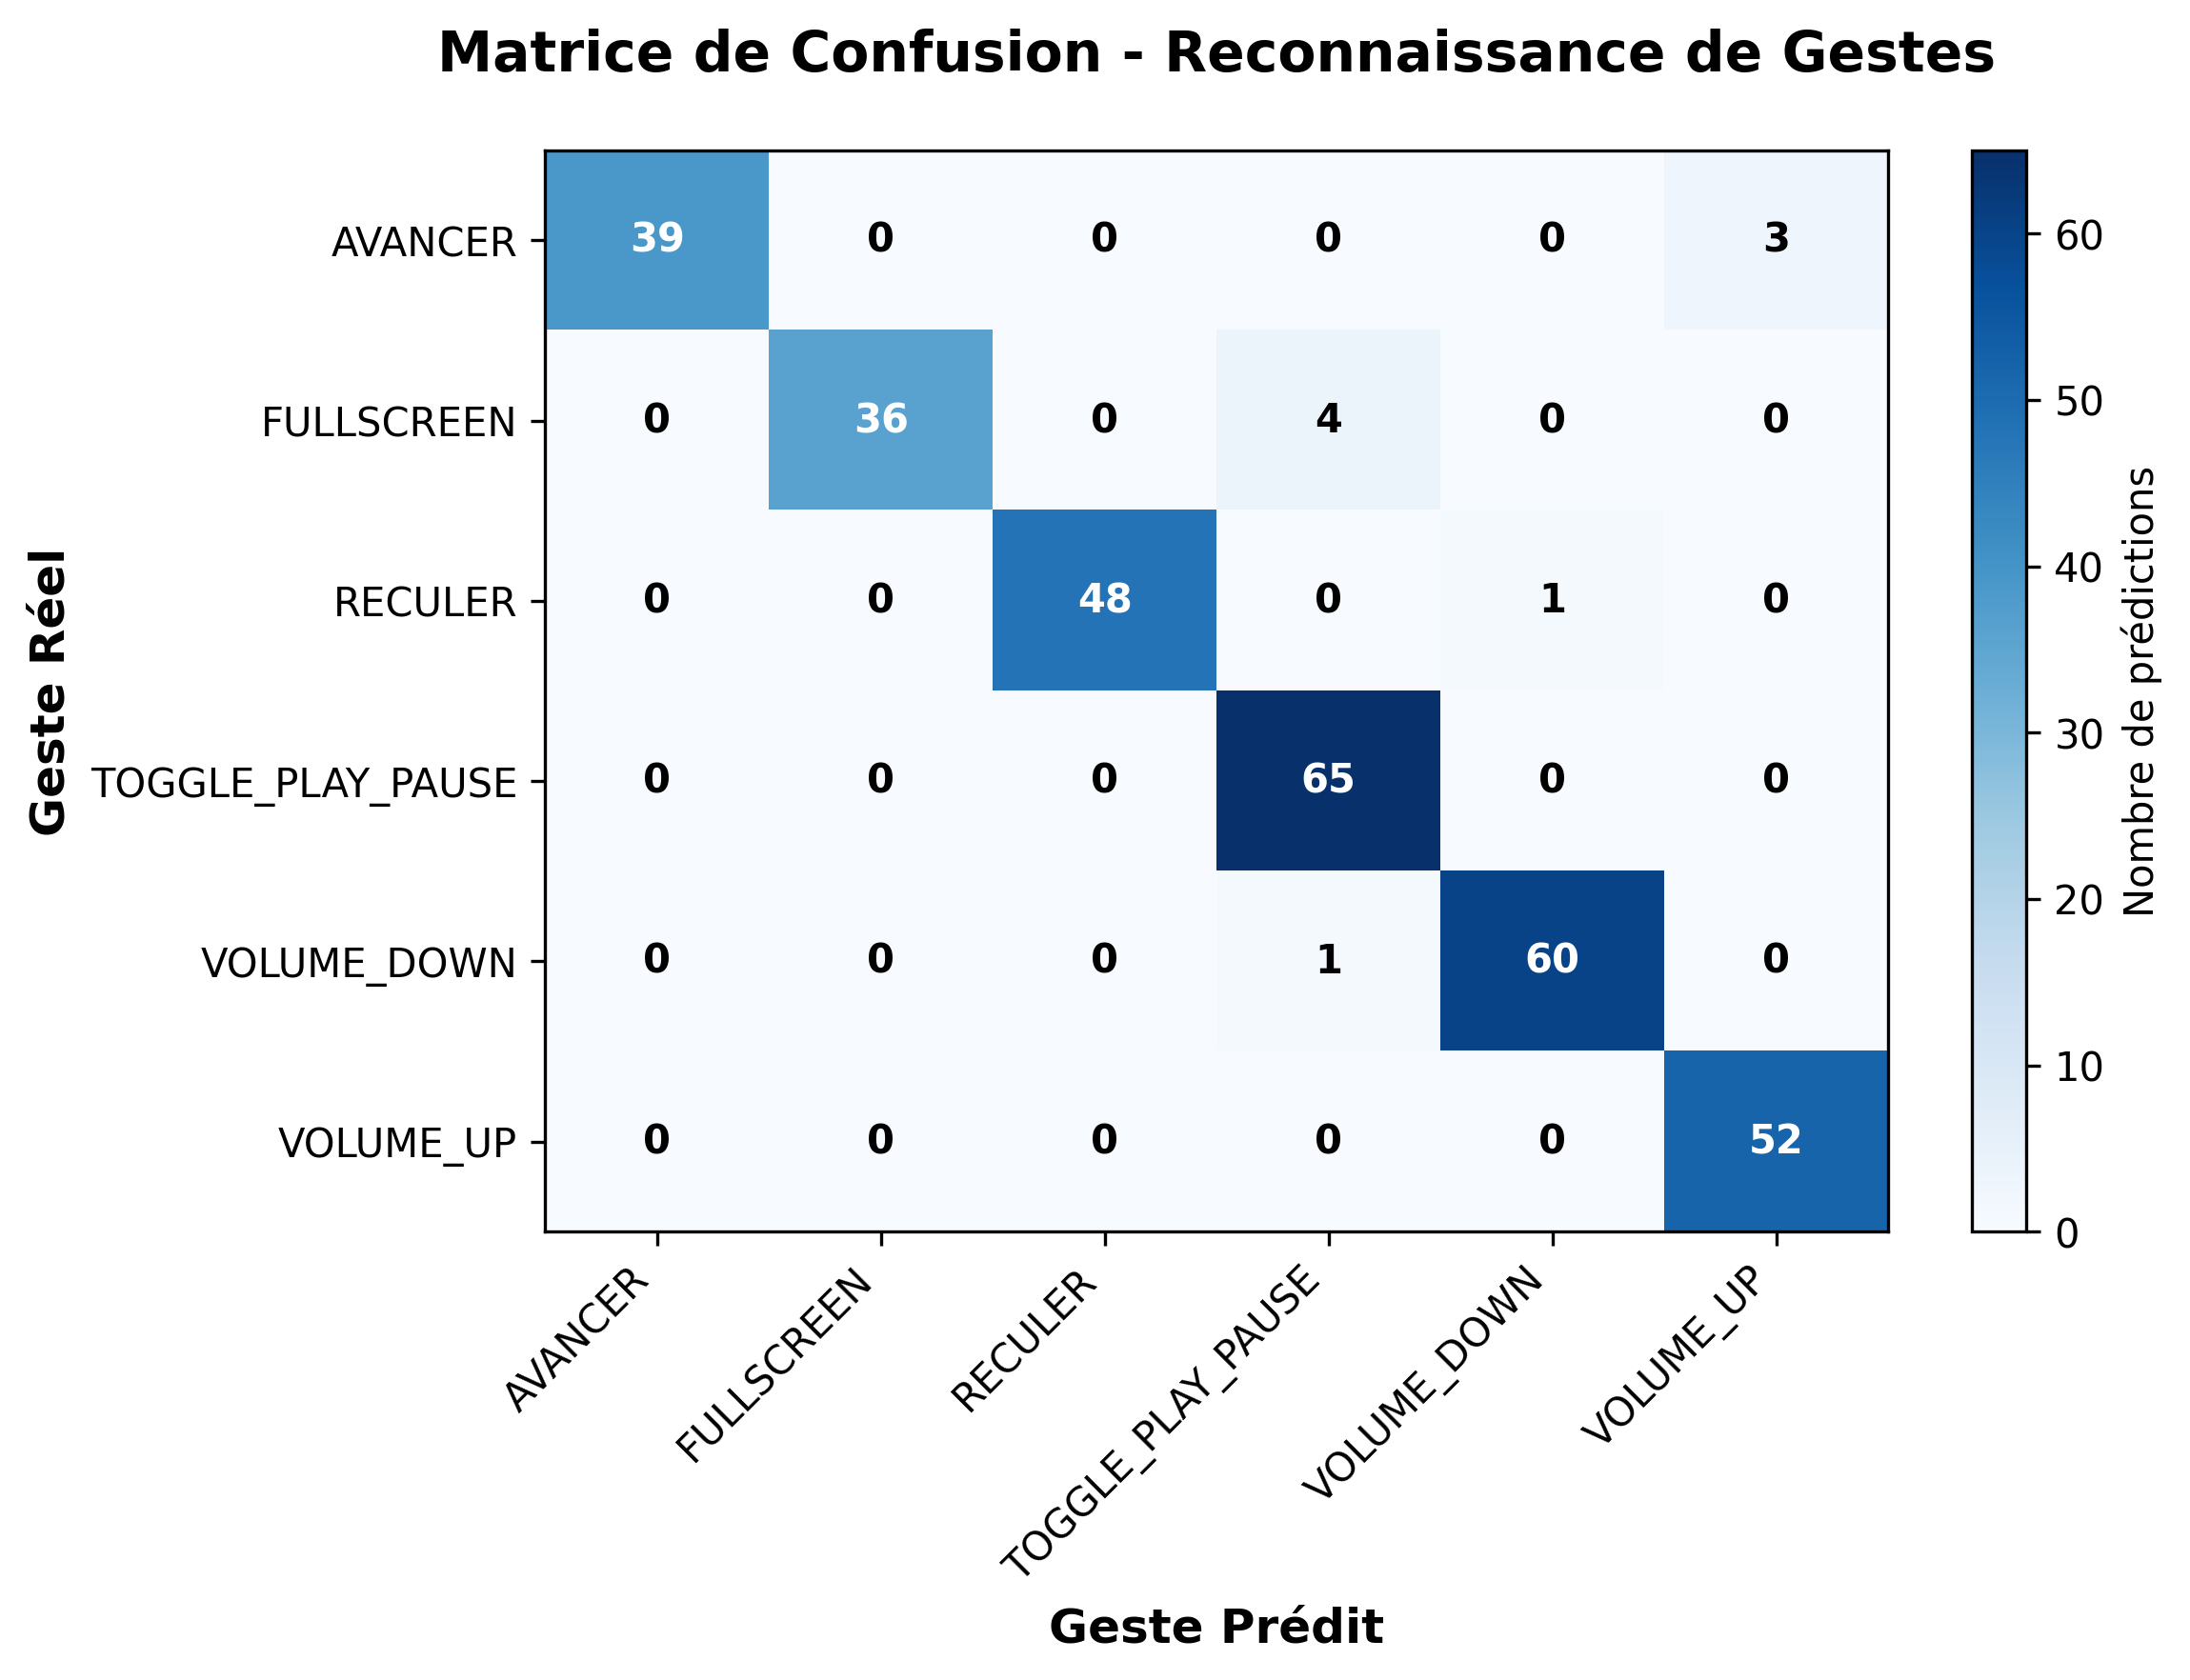
\includegraphics[width=0.8\textwidth]{../confusion_matrix_20251204_202545.png}
    \caption{Matrice de confusion des gestes reconnus}
    \label{fig:confusion}
\end{figure}

La matrice de confusion indique le nombre d'occurrences de chaque geste réel (lignes) prédit comme chaque geste (colonnes). La plupart des gestes sont correctement reconnus, avec de rares confusions : ``Avancer'' a été interprété 3 fois comme ``Volume\_Up'', et ``Fullscreen'' 4 fois comme ``Reculer''. Les autres gestes présentent une reconnaissance quasi parfaite.

\section{Améliorations futures suggérées}

Plusieurs axes d'amélioration pourraient être explorés pour renforcer les performances et l'utilité du système :

\begin{itemize}
    \item \textbf{Optimisation des seuils de détection} : Affiner davantage les seuils et ratios pour réduire les confusions entre gestes similaires, notamment entre les gestes de navigation (AVANCER/RECULER) et les gestes de volume (VOLUME\_UP/VOLUME\_DOWN).
    
    \item \textbf{Robustesse aux conditions d'éclairage} : Améliorer la détection dans différents environnements d'éclairage et distances de capture pour assurer une fiabilité optimale dans diverses conditions d'utilisation.
    
    \item \textbf{Approches alternatives de classification} : Explorer l'utilisation de modèles d'apprentissage automatique (réseaux de neurones) si les performances des règles heuristiques s'avèrent insuffisantes pour des gestes plus complexes.
    
    \item \textbf{Support multi-mains} : Étendre le système pour reconnaître des gestes impliquant les deux mains simultanément, permettant des commandes plus complexes et expressives.
    
    \item \textbf{Intégration avec des lecteurs vidéo externes} : Développer des interfaces de communication avec des lecteurs vidéo populaires (VLC, Windows Media Player) via des APIs ou des commandes système pour une compatibilité élargie.
\end{itemize}

\newpage

\section*{Références}

\begin{itemize}
    \item MediaPipe Hands Documentation. \url{https://google.github.io/mediapipe/solutions/hands}
    \item OpenCV Documentation. \url{https://docs.opencv.org/}
    \item PySide6 Documentation. \url{https://doc.qt.io/qtforpython/}
    \item Lugaresi, C., et al. (2019). MediaPipe: A Framework for Building Perception Pipelines.
\end{itemize}

\end{document}

